\documentclass[aspectratio=169]{beamer}
\usetheme{Madrid}
\usepackage[utf8]{inputenc}
\usepackage{graphicx}
\usepackage{amsmath}
\usepackage{booktabs}
\usepackage{tikz}
\usetikzlibrary{arrows.meta,positioning,shapes,fit,calc}

% App-like dark theme colors (Tailwind slate + cyan/indigo accents)
% Theme toggle: set to \lightthemetrue for light background
\newif\iflighttheme
\lightthemetrue

% Color palette
\definecolor{slate900}{HTML}{0F172A}
\definecolor{slate800}{HTML}{1E293B}
\definecolor{slate700}{HTML}{334155}
\definecolor{slate200}{HTML}{E2E8F0}
\definecolor{slate100}{HTML}{F8FAFC}
\definecolor{cyan400}{HTML}{22D3EE}
\definecolor{indigo400}{HTML}{818CF8}

% Beamer color setup matching app UI, light/dark aware
\iflighttheme
  \setbeamercolor{background canvas}{bg=slate100}
  \setbeamercolor{normal text}{fg=slate900}
  \setbeamercolor{frametitle}{fg=slate900,bg=slate200}
  \setbeamercolor{title}{fg=slate900}
  \setbeamercolor{subtitle}{fg=slate800}
  \setbeamercolor{structure}{fg=indigo400}
  \setbeamercolor{block title}{fg=slate900,bg=slate200}
  \setbeamercolor{block body}{fg=slate900,bg=slate100}
  \setbeamercolor{itemize item}{fg=indigo400}
\else
  \setbeamercolor{background canvas}{bg=slate900}
  \setbeamercolor{normal text}{fg=slate100}
  \setbeamercolor{frametitle}{fg=slate100,bg=slate800}
  \setbeamercolor{title}{fg=slate100}
  \setbeamercolor{subtitle}{fg=slate100}
  \setbeamercolor{structure}{fg=cyan400}
  \setbeamercolor{block title}{fg=slate100,bg=slate700}
  \setbeamercolor{block body}{fg=slate100,bg=slate800}
  \setbeamercolor{itemize item}{fg=cyan400}
\fi
\setbeamertemplate{navigation symbols}{}

\title{GeoAuPredict (GAP): Deep Learning for Geospatial Prediction of Gold}
\subtitle{Final Project — Deep Learning Course}
\author{Edward Calderón \& Team}
\date{\today}

\begin{document}

\frame{\titlepage}

\begin{frame}{Motivation and Problem Statement}
  \begin{itemize}
    \item Why geospatial prediction of gold is relevant (exploration, cost, risk).
    \item Traditional approaches: surveys, interpolation, geostatistics.
    \item Challenges: heterogeneous data, spatial autocorrelation, missingness.
    \item Our goal: learn from multi-modal geospatial data to predict Au occurrence.
  \end{itemize}
\end{frame}

\begin{frame}{Data Ingestion and Preprocessing}
  \begin{itemize}
    \item Sources: DEM, remote sensing indices, geology layers, geochemical assays, distances to structures.
    \item CRS harmonization, resampling, study area clipping, normalization.
    \item Spatially aware splits; class balance checks.
  \end{itemize}
\end{frame}

\begin{frame}{Exploratory Data Analysis}
  \begin{itemize}
    \item Correlations and distributions; outliers and missingness.
    \item Spatial plots of assays and features; clustering and hotspots.
    \item Early insights to guide feature engineering.
  \end{itemize}
\end{frame}

\begin{frame}{Pipeline Flow}
  \centering
  \resizebox{!}{0.78\textheight}{
% Auto-generated by generate_diagrams.py
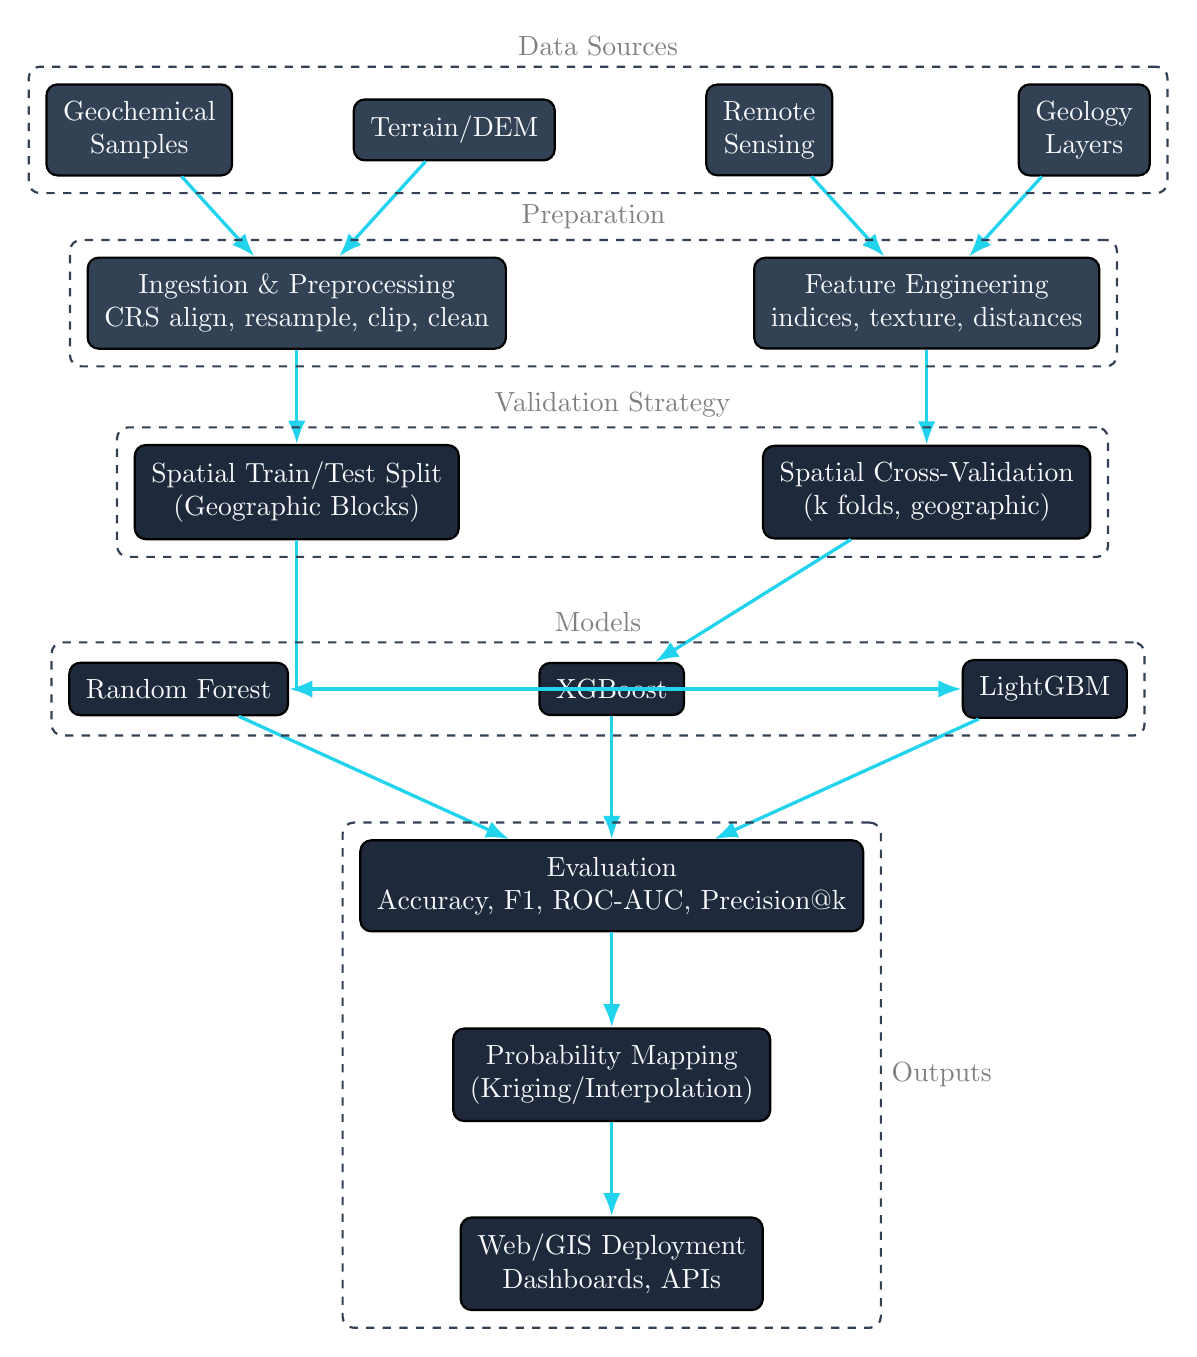
\begin{tikzpicture}[node distance=1.6cm]
  % Styles
  \tikzset{
    block/.style={draw, rounded corners, thick, align=center, fill=slate800, text=slate100, inner sep=6pt},
    data/.style={draw, rounded corners, thick, align=center, fill=slate700, text=slate100, inner sep=6pt},
    process/.style={draw, rounded corners, thick, align=center, fill=slate700, text=slate100, inner sep=6pt},
    result/.style={draw, rounded corners, thick, align=center, fill=slate800, text=slate100, inner sep=6pt},
    dashedblock/.style={draw=slate700, rounded corners, thick, align=center, dashed, inner sep=6pt},
    line/.style={-Latex, very thick, draw=cyan400},
  }

  % Row 1: Data sources (explicit coordinates to avoid overlap)
  \node[data] (geochem) at (0,0) {Geochemical\\Samples};
  \node[data] (terrain) at (4,0) {Terrain/DEM};
  \node[data] (remote)  at (8,0) {Remote\\Sensing};
  \node[data] (geology) at (12,0) {Geology\\Layers};

  % Row 2
  \node[process] (ingest) at (2,-2.2) {Ingestion \& Preprocessing\\CRS align, resample, clip, clean};
  \node[process] (feat)   at (10,-2.2) {Feature Engineering\\indices, texture, distances};

  % Row 3
  \node[block] (split) at (2,-4.6) {Spatial Train/Test Split\\(Geographic Blocks)};
  \node[block] (cv)    at (10,-4.6) {Spatial Cross-Validation\\(k folds, geographic)};

  % Row 4: Models
  \node[block] (rf)   at (0.5,-7.1) {Random Forest};
  \node[block] (xgb)  at (6.0,-7.1) {XGBoost};
  \node[block] (lgbm) at (11.5,-7.1) {LightGBM};

  % Row 5
  \node[result] (eval)    at (6.0,-9.6) {Evaluation\\Accuracy, F1, ROC-AUC, Precision@k};
  \node[result] (mapping) at (6.0,-12.0) {Probability Mapping\\(Kriging/Interpolation)};
  \node[result] (deploy)  at (6.0,-14.4) {Web/GIS Deployment\\Dashboards, APIs};

  % Edges
  \draw[line] (geochem) -- (ingest);
  \draw[line] (terrain) -- (ingest);
  \draw[line] (remote)  -- (feat);
  \draw[line] (geology) -- (feat);
  \draw[line] (ingest) -- (split);
  \draw[line] (feat)   -- (cv);
  \draw[line] (split)  |- (rf);
  \draw[line] (cv)     -- (xgb);
  \draw[line] (split)  |- (lgbm);
  \draw[line] (rf)  -- (eval);
  \draw[line] (xgb) -- (eval);
  \draw[line] (lgbm) -- (eval);
  \draw[line] (eval) -- (mapping);
  \draw[line] (mapping) -- (deploy);

  % Group boxes
  \node[dashedblock, fit=(geochem) (terrain) (remote) (geology), label={[gray]above:Data Sources}] {};
  \node[dashedblock, fit=(ingest) (feat), label={[gray]above:Preparation}] {};
  \node[dashedblock, fit=(split) (cv), label={[gray]above:Validation Strategy}] {};
  \node[dashedblock, fit=(rf) (xgb) (lgbm), label={[gray]above:Models}] {};
  \node[dashedblock, fit=(eval) (mapping) (deploy), label={[gray]right:Outputs}] {};
\end{tikzpicture}
}
\end{frame}

\begin{frame}{Modeling Approach}
  \begin{itemize}
    \item Tree ensembles: Random Forest, XGBoost, LightGBM (tabular geospatial features).
    \item Spatial cross-validation (geographic blocks) to assess generalization.
    \item Probability mapping via interpolation; uncertainty estimation.
  \end{itemize}
\end{frame}

\begin{frame}{Model Architecture (Ensemble)}
  \centering
  \resizebox{\textwidth}{!}{
% Auto-generated by generate_diagrams.py
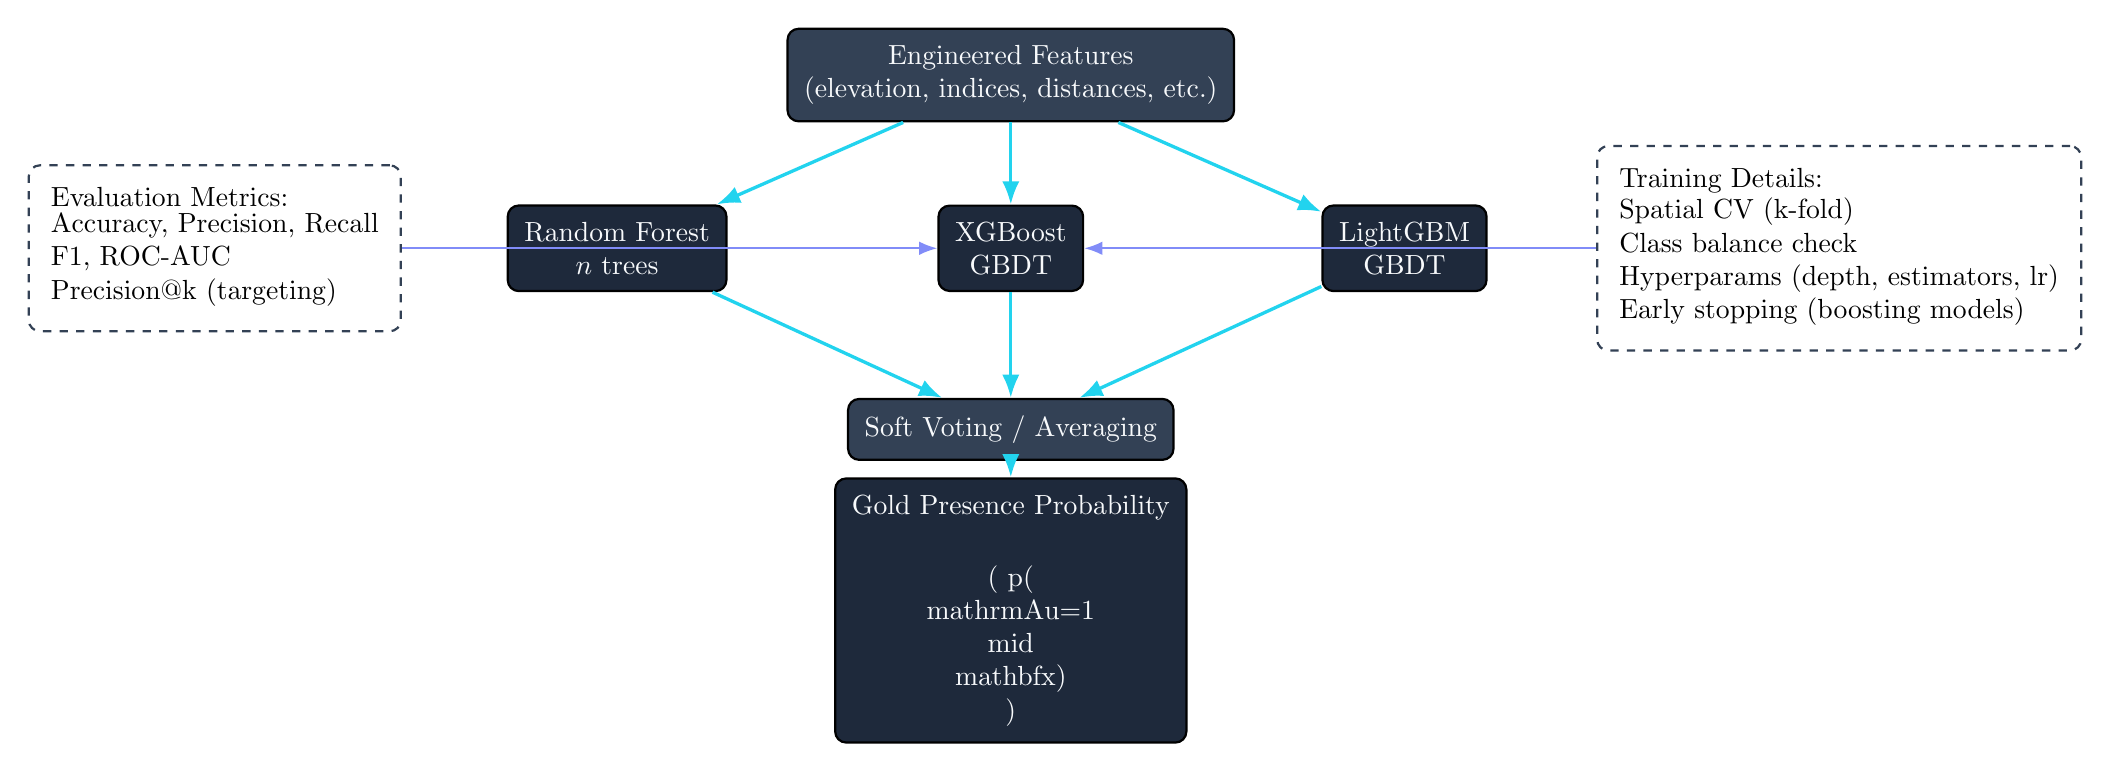
\begin{tikzpicture}[node distance=1.5cm]
  % Styles
  \tikzset{
    block/.style={draw, rounded corners, thick, align=center, fill=slate800, text=slate100, inner sep=6pt},
    data/.style={draw, rounded corners, thick, align=center, fill=slate700, text=slate100, inner sep=6pt},
    process/.style={draw, rounded corners, thick, align=center, fill=slate700, text=slate100, inner sep=6pt},
    result/.style={draw, rounded corners, thick, align=center, fill=slate800, text=slate100, inner sep=6pt},
    dashedblock/.style={draw=slate700, rounded corners, thick, align=center, dashed, inner sep=6pt},
    line/.style={-Latex, very thick, draw=cyan400},
    thinlink/.style={-Latex, thick, draw=indigo400},
  }

  % Inputs (fixed spacing)
  \node[data] (features) at (0,0) {Engineered Features\\(elevation, indices, distances, etc.)};

  % Base learners row
  \node[block] (rf)   at (-5,-2.2) {Random Forest\\$n$ trees};
  \node[block] (xgb)  at (0,-2.2)  {XGBoost\\GBDT};
  \node[block] (lgbm) at (5,-2.2)  {LightGBM\\GBDT};

  % Ensemble and output
  \node[process] (ens)  at (0,-4.5) {Soft Voting / Averaging};
  \node[result]  (proba) at (0,-6.8) {Gold Presence Probability\\[2pt] \\( p(\\mathrm{Au}=1\\mid \\mathbf{x}) \\)};

  % Links
  \draw[line] (features) -- (rf);
  \draw[line] (features) -- (xgb);
  \draw[line] (features) -- (lgbm);
  \draw[line] (rf) -- (ens);
  \draw[line] (xgb) -- (ens);
  \draw[line] (lgbm) -- (ens);
  \draw[line] (ens) -- (proba);

  % Side panels
  \node[dashedblock, right=6.5cm of xgb, align=left, inner sep=8pt] (trainbox) {Training Details:\\
    \begin{tabular}{@{}l@{}}
      Spatial CV (k-fold)\\
      Class balance check\\
      Hyperparams (depth, estimators, lr)\\
      Early stopping (boosting models)
    \end{tabular}
  };

  \node[dashedblock, left=6.8cm of xgb, align=left, inner sep=8pt] (evalbox) {Evaluation Metrics:\\
    \begin{tabular}{@{}l@{}}
      Accuracy, Precision, Recall\\
      F1, ROC-AUC\\
      Precision@k (targeting)
    \end{tabular}
  };

  \draw[thinlink] (trainbox.west) -- ++(-0.7,0) |- (xgb);
  \draw[thinlink] (evalbox.east) -- ++(0.7,0) |- (xgb);
\end{tikzpicture}
}
\end{frame}

\begin{frame}{Training \& Validation}
  \begin{itemize}
    \item Metrics: Accuracy, Precision, Recall, F1, ROC-AUC, Precision@k.
    \item Early stopping for boosting models; hyperparameter sanity checks.
    \item Spatial CV (geographic blocks) for honest generalization.
    \item Key results from notebooks:
      \begin{itemize}
        \item \textbf{LightGBM (best base)}: AUC = \textbf{0.9243}
        \item \textbf{Voting Ensemble (production)}: AUC = \textbf{0.9208} (spatially separated test)
        \item \textbf{Spatial Blocks AUC}: \textbf{0.86} (geographic CV)
      \end{itemize}
  \end{itemize}
\end{frame}

\begin{frame}{Results Summary}
  \begin{itemize}
    \item \textbf{Best base model}: LightGBM — AUC \textbf{0.9243}
    \item \textbf{Production model}: Voting Ensemble — AUC \textbf{0.9208} (spatially separated test)
    \item \textbf{Spatial Blocks AUC (CV)}: \textbf{0.86} — honest, geography-aware estimate
    \item Precision@k supports efficient targeting (top areas).\footnotesize{\,Demo runs show high P@10; full report omitted here}
  \end{itemize}
\end{frame}

\begin{frame}{Comparison with Classical Methods}
  \begin{itemize}
    \item Baselines: kriging, logistic regression, WoE, SVM (literature typical AUC \(\approx 0.82\)).
    \item \textbf{Improvement}: +\(\sim\)\textbf{22\%} AUC over best classical (0.82 \(\to\) 0.9208/0.9243).
    \item Strengths: DL/ensembles capture non-linear, multi-modal interactions.
    \item Limitations: classical methods often assume stationarity/linearity.
  \end{itemize}
\end{frame}

\begin{frame}{Ablation \& Sensitivity}
  \begin{itemize}
    \item Feature importance / permutation importance; remove/keep studies.
    \item Hyperparameters: depth, estimators, learning rate.
    \item Robustness: spatial CV folds, noise perturbations.
  \end{itemize}
\end{frame}

\begin{frame}{Deployment \& Use Cases}
  \begin{itemize}
    \item Deployment: web dashboards, GIS export, APIs.
    \item Use cases: guide field sampling; prioritize zones; decision support.
    \item Limitations: domain shift, data availability, generalization.
  \end{itemize}
\end{frame}

\begin{frame}{Q\&A Strategy (Judge Questions)}
  \small
  \begin{tabular}{p{0.48\textwidth} p{0.48\textwidth}}
  \textbf{Why DL vs geostatistics?} & Non-linear interactions; heterogeneous modalities; scale. Classical often assume stationarity / linearity. \\
  \textbf{Avoiding overfitting?} & Spatial CV; regularization; early stopping; non-contiguous holdouts; augmentation. \\
  \textbf{Interpretability?} & Feature importance, SHAP, LRP, surrogate models; spatial attribution maps. \\
  \textbf{Transferability?} & Domain shift awareness; fine-tuning; multi-region training; domain adaptation. \\
  \textbf{Uncertainty?} & If absent: propose MC-dropout, ensembles, quantile reg.; report as future work. \\
  \textbf{Compare to SOTA?} & Cite TorchGeo/remote sensing DL; compare metrics/approach; highlight novelty. \\
  \textbf{Limitations?} & Overfitting risk; sparse labels; sensor noise; domain shift; interpretability. \\
  \textbf{Operational integration?} & Data ingestion pipeline; real-time inference; GIS integration; feedback loop. \\
  \end{tabular}
\end{frame}

\begin{frame}{Conclusions}
  \begin{itemize}
    \item Novelty: multi-modal integration, spatial CV, probability mapping.
    \item Impact: reduce exploration costs; improve targeting; scalable pipeline.
    \item Future: uncertainty quantification; domain adaptation; explainability.
  \end{itemize}
\end{frame}

\begin{frame}{Questions}
  \centering\Large Thank you!\\[0.5cm]Questions welcome.\\[0.6cm]
  \href{https://edwardcalderon.github.io/GeoAuPredict/login}{\beamergotobutton{Demo}}\\[0.4cm]
  \small \href{https://github.com/edwardcalderon/GeoAuPredict/}{github.com/edwardcalderon/GeoAuPredict}
\end{frame}

\end{document}

